\begin{name}
	{\tenchude}{\tendethi}{LỚP TOÁN THẦY PHÁT}{\thoigian}
\end{name}
\setcounter{ex}{0}\setcounter{bt}{0}
\Opensolutionfile{ans}[ans/ans-2-TT-25-YenLac2-VinhPhuc-L3-23]
\setcounter{ex}{0}


\begin{ex}%[Đề thi thử THPT Yên Lạc 2 Vĩnh Phúc]%[Nguyễn Thành Nhân, 12EX-5-2223]%[2H1Y3-2]
	Thể tích của khối hộp chữ nhật có các kích thước $ 4 $, $ 5 $, $ 6 $ là
	\choice
	{$ 20 $}
	{$ 40 $}
	{$ 60 $}
	{\True $ 120 $}
	\loigiai{
		Ta có thể tích khối hộp chữ nhật là $ V=abc=4\cdot5\cdot6=120 $.
	}
\end{ex}

\begin{ex}%[Đề thi thử THPT Yên Lạc 2 Vĩnh Phúc]%[Nguyễn Thành Nhân, 12EX-5-2223]%[2H3Y1-3] 
	Trong không gian $ Oxyz $, cho mặt cầu $ (S) $ có phương trình $ (x-2)^2+(y+1)^2+(z+2)^2=4 $. Tâm và bán kính của mặt cầu là
	\choice
	{$ I(-2;1;2) $, $ R=2 $}
	{$ I(2;-1;-2) $, $ R=4 $}
	{\True $ I(2;-1;-2) $, $ R=2 $}
	{$ I(2;-1;-2) $, $ R=16 $}
	\loigiai{
		Mặt cầu $ (S) $ có tâm $ I(2;-1;-2) $ và bán kính  $ R=\sqrt{4}=2 $.
	}
\end{ex}


\begin{ex}%[Đề thi thử THPT Yên Lạc 2 Vĩnh Phúc]%[Nguyễn Thành Nhân, 12EX-5-2223]%[2D2Y4-3]
	Có bao nhiêu giá trị nguyên của $ a $ để hàm số $ y=(3a-11)^x $ nghịch biến trên $ \mathbb{R} $?
	\choice
	{\True $ 0 $}
	{$ 1 $}
	{$ 2 $}
	{$ 3 $}
	\loigiai{
	Hàm số 	$ y=(3a-11)^x $ nghịch biến trên $ \mathbb{R} $ khi $ 0<3a-11<1\Leftrightarrow \dfrac{11}{3}<a<\dfrac{12}{3} $.\\
	Do đó không có giá trị nguyên của $ a $ thỏa yêu cầu đề bài.
	}
\end{ex}

\begin{ex}%[Đề thi thử THPT Yên Lạc 2 Vĩnh Phúc]%[Nguyễn Thành Nhân, 12EX-5-2223]%[1D2Y1-1]
	Có bao nhiêu cách lấy ra một quả cầu từ hộp có chứa $ 14 $ quả cầu màu đỏ và $ 15 $ quả cầu màu vàng?
	\choice
	{$ 210 $}
	{\True $ 29 $}
	{$ 14 $}
	{$ 15 $}
	\loigiai{
	\begin{itemize}
		\item  Phương án 1: Lấy $ 1 $ quả cầu màu đỏ có $ 14 $ cách.
		\item Phương án 2: Lấy $ 1 $ quả cầu màu vàng có $ 15 $ cách.
	\end{itemize}	
Theo quy tắc cộng ta có $ 14+15=29 $ cách.
	}
\end{ex}

\begin{ex}%[Đề thi thử THPT Yên Lạc 2 Vĩnh Phúc]%[Nguyễn Thành Nhân, 12EX-5-2223]%[2H3B2-3]
	Trong không gian $ Oxyz $, mặt phẳng song song với mặt phẳng $ Oxy $ và đi qua điểm $ A(2;2;2) $ có phương trình là
	\choice
	{$ y-2=0 $}
	{$ x+y+z-1=0 $}
	{\True $ z-2=0 $}
	{$ x-2=0 $}
	\loigiai{
		Phương trình mặt phẳng $ Oxy $ là $ z=0 $.\\
		Phương trình mặt phẳng song song với $ Oxy $ có dạng $ z+d=0 $, $ (d\ne 0 )$.\\
		Vì mặt phẳng $ z+d=0 $ đi qua $ A(2;2;2) $ suy ra $ d=-2 $. Vậy $ z-2=0 $ là mặt phẳng cần tìm.
	}
\end{ex}

\begin{ex}%[Đề thi thử THPT Yên Lạc 2 Vĩnh Phúc]%[Nguyễn Thành Nhân, 12EX-5-2223]%[2D1Y5-4]
	Cho hàm số $ y=x^3-3x+2 $ có đồ thị là $ (C) $. Số giao điểm của $ (C) $ và trục hoành là
	\choice
	{$ 3 $}
	{$ 1 $}
	{\True $ 2 $}
	{$ 0 $}
	\loigiai{
		Xét phương trình hoành độ giao điểm của $ (C) $ và trục hoành là $$ x^3-3x+2=0\Leftrightarrow (x+2)(x-1)^2=0\Leftrightarrow \hoac{&x=-2\\&x=1.} $$
		Phương trình hoành độ giao điểm có $ 2 $ nghiệm nên $ (C) $ cắt trục hoành tại $ 2 $ điểm.
	}
\end{ex}

\begin{ex}%[Đề thi thử THPT Yên Lạc 2 Vĩnh Phúc]%[Nguyễn Thành Nhân, 12EX-5-2223]%[2D3Y2-1]
	Cho $ \displaystyle\int\limits_{-1}^{2} f(x)\mathrm{\,d}x=3 $, $ \displaystyle\int\limits_{-1}^{2} g(x)\mathrm{\,d}x=-1 $. Khi đó $ I=\displaystyle\int\limits_{-1}^{2} [x+2f(x)-3g(x)]\mathrm{\,d}x $ bằng
	\choice
	{$ 10 $}
	{\True $ \dfrac{21}{2} $}
	{$ \dfrac{19}{2} $}
	{$ \dfrac{17}{2} $}
	\loigiai{
	Ta có 	$ I=\displaystyle\int\limits_{-1}^{2} [x+2f(x)-3g(x)]\mathrm{\,d}x=\displaystyle\int\limits_{-1}^{2}x \mathrm{\,d}x+2\displaystyle\int\limits_{-1}^{2} f(x)\mathrm{\,d}x-3\displaystyle\int\limits_{-1}^{2}g(x) \mathrm{\,d}x=\dfrac{x^2}{2}\bigg|_{-1}^{2}+2\cdot 3-3\cdot(-1)=\dfrac{21}{2}$.
	}
\end{ex}
\begin{ex}%[Đề thi thử THPT Yên Lạc 2 Vĩnh Phúc]%[Nguyễn Thành Nhân, 12EX-5-2223]%[2D1Y2-1]
	Số cực trị của hàm số $ f(x)=\dfrac{x-2023}{2x+1} $ là
\choice
{$ 2 $}
{\True $ 0 $}
{$ 1 $}
{$ 3 $}
\loigiai{
Ta có $ f'(x)=\dfrac{4047}{(2x+1)^2}>0,\forall x\in \mathbb{R} $ suy ra hàm số $ y=f(x) $ đồng biến trên từng khoảng xác định.\\
Suy ra hàm số $ y=f(x) $ không có cực trị.
}
\end{ex}

\begin{ex}%[Đề thi thử THPT Yên Lạc 2 Vĩnh Phúc]%[Nguyễn Thành Nhân, 12EX-5-2223]%[1D5B2-2]
	Cho hàm số $ (C)\colon y=x^3+3x^2 $. Phương trình tiếp tuyến của $ (C) $ tại điểm $ M(1;4) $ là  
	\choice
	{\True $ y=9x-5 $}
	{$ y=-9x+5 $}
	{$ y=-9x-5 $}
	{$ y=9x+5 $}
	\loigiai{
	Ta có $ y'=f'(x)=3x^2+6x $.\\
	Gọi phương trình tiếp tuyến có dạng $ y=f'(x_0)(x-x_0)+y_0 $.\\
	Vì tiếp tuyến của $ (C) $ tại $ M(1;4) $ suy ra $ x_0=1 $ và $ y_0=4 $ do đó  $ f'(1)=9 $.\\
	Vậy phương trình tiếp tuyến là $ y=9(x-1)+4\Leftrightarrow y=9x-5 $.	
	}
\end{ex}



\begin{ex}%[Đề thi thử THPT Yên Lạc 2 Vĩnh Phúc]%[Nguyễn Thành Nhân, 12EX-5-2223]%[2H3Y1-2]
	Trong không gian với hệ trục tọa độ $ Oxyz $, cho hai véc-tơ $ \overrightarrow{u}=(2;3;-1) $ và $ \overrightarrow{v}=(5;-4;m) $. Tìm $ m $ để $ \overrightarrow{u}\perp \overrightarrow{v} $.
	\choice
	{$ m=2 $}
	{$ m=4 $}
	{$ m=-4 $}
	{\True $ m=-2 $}
	\loigiai{
	Để 	$ \overrightarrow{u}\perp \overrightarrow{v} $ thì $ \overrightarrow{u}\cdot \overrightarrow{v}=0 \Leftrightarrow 2\cdot 5+3\cdot (-4)+(-1)\cdot m=0\Leftrightarrow m=-2$.
	}
\end{ex}

\begin{ex}%[Đề thi thử THPT Yên Lạc 2 Vĩnh Phúc]%[Nguyễn Thành Nhân, 12EX-5-2223]%[2D2Y4-2]
	Cho hàm số $ f(x)=\ln(x^2+1) $. Giá trị của $ f'(2) $ bằng
	\choice
	{$ 2 $}
	{\True $ \dfrac{4}{5} $}
	{$ \dfrac{4}{2\ln5} $}
	{$ \dfrac{4}{3\ln2} $}
	\loigiai{
	Ta có $ f'(x)=\dfrac{2x}{x^2+1}\Rightarrow f'(2)=\dfrac{4}{5} $.	
	}
\end{ex}

\begin{ex}%[Đề thi thử THPT Yên Lạc 2 Vĩnh Phúc]%[Nguyễn Thành Nhân, 12EX-5-2223]%[2H2Y1-2]
	Cho hình trụ có diện tích xung quanh $ 50\pi $ và độ dài đường sinh bằng đường kính của đường tròn đáy. Bán kính $ r $ của đường tròn đáy là
	\choice
	{$ r=\dfrac{5}{2} $}
	{$ r=5 $}
	{\True $ r=\dfrac{5\sqrt{2}}{2} $}
	{$ r=5\sqrt{2} $}
	\loigiai{ Do đường kính bằng đường sinh nên $ 2r=d=l $.\\
	Ta có diện tích xung quanh của hình trụ là $ S=2\pi r l\Leftrightarrow 50\pi =2\pi r\cdot 2r \Leftrightarrow r^2=\dfrac{25}{2}\Rightarrow r=\dfrac{5\sqrt{2}}{2}$.
	}
\end{ex}


\begin{ex}%[Đề thi thử THPT Yên Lạc 2 Vĩnh Phúc]%[Nguyễn Thành Nhân, 12EX-5-2223]%[2D3B3-1]
	Diện tích hình phẳng giới hạn bởi đồ thị hàm số $ y=(x-2)^2 -1$, trục hoành và hai đường thẳng  $ x=1 $, $ x=2 $ bằng
	\choice
	{\True $ \dfrac{2}{3} $}
	{$ \dfrac{7}{3} $}
	{$ \dfrac{1}{3} $}
	{$ \dfrac{3}{2} $}
	\loigiai{
	Ta có $ (x-2)^2 -1=0\Leftrightarrow x^2-4x+3=0 \Leftrightarrow \hoac{&x=1\\&x=3.} $\\
	Bảng xét dấu 
	\begin{center}
		
\begin{tikzpicture}[font=\footnotesize,line join=round, line cap=round, >=stealth,scale=1]
		\tkzTabInit[nocadre=false,lgt=2.2,espcl=2.5,deltacl=0.6] 
		{$x$ /0.6,$x^2-4x+3$ /0.6}
		{$-\infty$,$1$,$3$,$+\infty$}
		\tkzTabLine{ ,+,$0$,-,$0$,+, }
		\end{tikzpicture}
	\end{center}
	Ta có diện tích hình phẳng được tính bởi công thức $$ \displaystyle\int\limits_{1}^{2} |(x-2)^2-1|\mathrm{\,d}x=-\displaystyle\int\limits_{1}^{2} (x^2-4x+3)\mathrm{\,d}x=-\left( \dfrac{x^3}{3}-2x^2+3x\right) \bigg|_1^2=\dfrac{2}{3}. $$
	}
\end{ex}

\begin{ex}%[Đề thi thử THPT Yên Lạc 2 Vĩnh Phúc]%[Nguyễn Thành Nhân, 12EX-5-2223]%[2D2B6-2]
	Tập nghiệm của bất phương trình $ (\sqrt{5}-2)^{x+1}>9-4\sqrt{5} $ là
	\choice
	{$ (1;+\infty) $}
	{$ (-1;-1) $}
	{$ (-\infty;1] $}
	{\True $ (-\infty;1) $}
	\loigiai{
	Ta có 
	\begin{eqnarray*}
		& & (\sqrt{5}-2)^{x+1}>9-4\sqrt{5}\\
		&\Leftrightarrow & (\sqrt{5}-2)^{x+1}>(\sqrt{5}-2)^2\\
		&\Leftrightarrow & x+1<2\Leftrightarrow x<1.
	\end{eqnarray*}
	}
\end{ex}




\begin{ex}%[Đề thi thử THPT Yên Lạc 2 Vĩnh Phúc]%[Nguyễn Thành Nhân, 12EX-5-2223]%[2D1B5-1]
	\immini{Cho đồ thị hàm số $ y=f'(x) $ như hình vẽ. Hàm số $y=f(x)$ đạt giá trị lớn nhất trên đoạn $ [1;3] $ tại $ x_0 $. Khi đó giá trị của $ x_0^2-3x_0+2023 $ bằng bao nhiêu?
		\choice
	{$ 2024 $}
	{$ 2023 $}
	{\True $ 2021 $}
	{$ 2022 $}}{\begin{tikzpicture}[font=\footnotesize,line join=round, line cap=round, >=stealth,scale=0.8]
		\tikzset{label style/.style={font=\footnotesize}}
		\draw[->] (-0.5,0)--(4,0) node[below left] {$x$};
		\draw[->] (0,-1.3)--(0,2) node[below left] {$y$};
		\fill (0,0) node [below left] {$O$} circle (1pt);
		\fill (1,0) node[below right]{$1$} circle (1pt);
		\fill (2,0) node[above]{$2$} circle (1pt);
		\fill (3,0) node[below right]{$3$} circle (1pt);
		\begin{scope}
		\clip (0.7,-0.8) rectangle (3.3,0.8);
		\draw[samples=200,domain=-1:5,smooth,variable=\x] plot (\x,{1*((\x)^3)-6*((\x)^2)+11*(\x)-6});
		\end{scope}
		\end{tikzpicture}}
	\loigiai{
		Từ đồ thị ta có bảng biến thiên của hàm số $y= f(x)$ là 
	\begin{center}
	
\begin{tikzpicture}[font=\footnotesize,line join=round, line cap=round, >=stealth,scale=1]
	\tkzTabInit[nocadre=false,lgt=1,espcl=2.5,deltacl=.6]
	{$x$/0.6,$y'$/0.6,$y$/2}
	{$-\infty$,$1$,$2$,$3$,$+\infty$}
	\tkzTabLine{,-,0,+,0,-,0,+}
	\tkzTabVar{+/$+\infty$,-/$ $,+/$ $,-/$ $,+/$+\infty$}
	\end{tikzpicture}
\end{center}
		Từ bảng biến thiên của hàm số $ y=f(x) $ suy ra $\max\limits_{x\in[1;3]} f(x)=f(2)$ suy ra $ x_0=2 $.\\
		Do đó $ x_0^2-3x_0+2023 =2021$.
	}
\end{ex}

\begin{ex}%[Đề thi thử THPT Yên Lạc 2 Vĩnh Phúc]%[Nguyễn Thành Nhân, 12EX-5-2223]%[2H2Y1-1]
	Thể tích khối nón có chiều cao $ h=3 $ bán kính $ r=4 $ bằng
	\choice
	{$ 12\pi $}
	{$ 48\pi $}
	{$ 4\pi $}
	{\True $ 16\pi $}
	\loigiai{
	Ta có thể tích khối nón là $ V=\dfrac{1}{3}\pi r^2h=\dfrac{1}{3}\cdot \pi \cdot 4^2\cdot 3=16\pi $.	
	}
\end{ex}

\begin{ex}%[Đề thi thử THPT Yên Lạc 2 Vĩnh Phúc]%[Nguyễn Thành Nhân, 12EX-5-2223]%[2H1B1-2]
	Cho hình chóp có số đỉnh là $ 2023 $, số cạnh của hình chóp đó là
	\choice
	{$ 1012 $}
	{\True $ 4044 $}
	{$ 4046 $}
	{$ 1011 $}
	\loigiai{
	Gọi $ n $ là số cạnh ở đáy của hình chóp.\\
	Suy ra số đỉnh của hình chóp là  $ n+1=2023\Leftrightarrow n=2022 $ suy ra số cạnh của hình chóp là $ 2n=4044 $.	
	}
\end{ex}

\begin{ex}%[Thi thử tốt nghiệp - THPT Yên Lạc 2-Vĩnh Phúc-23]%[Nguyễn Thành Nhân- EX6]%[2D1Y1-2]
\immini{
	Cho hàm số $y=f(x)$ có đồ thị như hình vẽ bên. Hàm số đồng biến trên khoảng nào?
	\choice
	{$(0;2)$}
	{\True $(-2;-1)$}
	{$(-2;0)$}
	{$(-1;1)$}}
	 {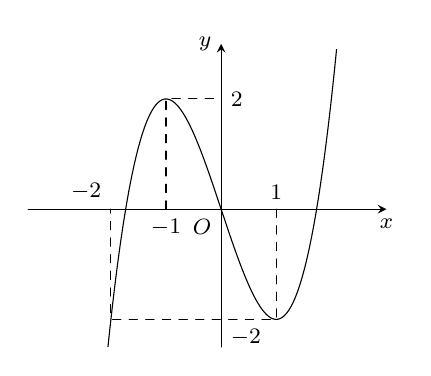
\begin{tikzpicture}[scale=0.7, font=\footnotesize,line join=round, line cap=round, >=stealth]
    \def\xt{-3.5} \def\xp{3} \def\yt{3} \def\yd{-2.5}
    \draw[->] (\xt,0)--(\xp,0) node [below]{$x$};
    \draw[->] (0,\yd)--(0,\yt) node [left]{$y$};
    \node at (0,0) [below left]{$O$};
    \clip (\xt,\yd) rectangle (\xp-0.1,\yt-0.1);
    \draw[smooth,samples=150,domain=-3:3] plot(\x,{(\x)^3-3*(\x)});
    \draw[dashed] (-1,0)node[below]{$-1$}|-(0,2)node[right]{$2$}
    (1,0)node[above]{$1$}|-(0,-2)node[below right]{$-2$}--(-2,-2)--(-2,0)node[above left]{$-2$};
    \end{tikzpicture}}
	\loigiai{
	Dựa vào đồ thị ta thấy hàm số đồng biến trên khoảng $(-2;-1)$. 
	}
\end{ex}
\begin{ex}%[Thi thử tốt nghiệp - THPT Yên Lạc 2-Vĩnh Phúc-23]%[Nguyễn Thành Nhân- EX6]%[2D3Y3-1]
\immini{
Gọi $S$ là diện tích hình phẳng giới hạn bởi các đường $y=f(x)$, trục hoành và hai đường thẳng $x=-3$, $x=2$ (như hình vẽ). Đặt $a=\displaystyle\int\limits_{-3}^1 f(x)\mathrm{\,d}x$, $b=\displaystyle\int\limits_{1}^2 f(x)\mathrm{\,d}x$. Mệnh đề nào sau đây đúng?
	\choice
	{$S=-a-b$}
	{$S=a+b$}
	{$S=a-b$}
	{\True $S=b-a$}}
	{\begin{tikzpicture}[>=stealth, font=\footnotesize, line join=round, line cap=round, scale=1]
	\draw[->] (-4,0) --(3,0) node[below]{$x$};
	\draw[->] (0,-3.5) --(0,1.5) node[left]{$y$};
	\draw (0,0) node[below left=-3pt]{$O$};
	\begin{scope}
	\clip (-4,-3.5) rectangle (3,1.5);
	\draw (-3,-3).. controls +(0:1) and +(180:0) .. (0,-1.2)
	.. controls +(0:0) and +(-120:0.4) .. (1,0)
	.. controls +(70:0.4) and +(130:0) .. (2,0.75);
	\end{scope}
	\draw[pattern = north west lines,draw=none] (-3,-3).. controls +(0:1) and +(180:0) .. (0,-1.2)
	.. controls +(0:0) and +(-120:0.4) .. (1,0)
	.. controls +(70:0.4) and +(130:0) .. (2,0.75)--(2,0)--(-3,0);
	\draw[dashed] (-3,0)--(-3,-3) (2,0)--(2,0.75);
	\foreach \p/\r in {-3/90,1/-90,2/-90}\fill (\p,0) circle (1.25pt) node[shift={(\r:2.5mm)}]{$\p$};
	\end{tikzpicture}}
	\loigiai{
	Ta có 
	\begin{eqnarray*}
	S&=&\displaystyle\int\limits_{-3}^2\left| f(x)\right|\mathrm{\,d}x=\displaystyle\int\limits_{-3}^1\left| f(x)\right|\mathrm{\,d}x+\displaystyle\int\limits_{1}^2\left| f(x)\right|\mathrm{\,d}x\\
	&=&-\displaystyle\int\limits_{-3}^1 f(x)\mathrm{\,d}x+\displaystyle\int\limits_{1}^2 f(x)\mathrm{\,d}x=-a+b.
	\end{eqnarray*}
	}
\end{ex}

\begin{ex}%[Thi thử tốt nghiệp - THPT Yên Lạc 2-Vĩnh Phúc-23]%[Nguyễn Thành Nhân- EX6]%[2H3Y1-1]
Trong không gian $Oxyz$, hình chiếu vuông góc của điểm $A(1;2;3)$ trên mặt phẳng $\left(Oxz\right)$ là
	\choice
	{$P(0;2;3)$}
	{\True $M(1;0;3)$}
	{$N(0;2;0)$}
	{$Q(1;2;0)$}
	\loigiai{
Hình chiếu vuông góc của điểm $A(1;2;3)$ trên mặt phẳng $\left(Oxz\right)$ là điểm $M(1;0;3)$.
	}
\end{ex}
\begin{ex}%[Thi thử tốt nghiệp - THPT Yên Lạc 2-Vĩnh Phúc-23]%[Nguyễn Thành Nhân- EX6]%[2D2B3-2]
	Cho $\log3=a$, $\log2=b$. Khi đó giá trị của $\log_{125}30$ được tính theo $a$, $b$ là 
	\choice
	{\True $\dfrac{1+a}{3(1-b)}$}
	{$\dfrac{4(3-a)}{3-b}$}
	{$\dfrac{a}{3+b}$}
	{$\dfrac{a}{3+a}$}
	\loigiai{
		Ta có
		\begin{eqnarray*}
		\log_{125}30&=& \dfrac{\log 30}{\log 125}=\dfrac{1+\log 3}{3\log 5}\\
		&=& \dfrac{1+\log3}{3\left(1-\log 2\right)}=\dfrac{1+a}{3(1-b)}.
		\end{eqnarray*}
	}
\end{ex}
\begin{ex}%[Thi thử tốt nghiệp - THPT Yên Lạc 2-Vĩnh Phúc-23]%[Nguyễn Thành Nhân- EX6]%[2D3B1-2]
	Nguyên hàm của $f(x)=\dfrac{2}{4x+3}$ là 
	\choice
	{$\displaystyle\int\limits \dfrac{2}{4x+3}\mathrm{\,d}x=2\ln \left|4x+3\right|+C$}
	{\True $\displaystyle\int\limits \dfrac{2}{4x+3}\mathrm{\,d}x=\dfrac{1}{2}\ln \left|4x+3\right|+C$}
	{$\displaystyle\int\limits \dfrac{2}{4x+3}\mathrm{\,d}x=\dfrac{1}{4}\ln \left|4x+3\right|+C$}
	{$\displaystyle\int\limits \dfrac{2}{4x+3}\mathrm{\,d}x=2\ln \left|2x+\dfrac{3}{2}\right|+C$}
	\loigiai{
		Ta có
		\begin{eqnarray*}
		\displaystyle\int\limits \dfrac{2}{4x+3}\mathrm{\,d}x=2\cdot \dfrac{1}{4}\ln \left|4x+3\right|+C=\dfrac{1}{2}\ln \left|4x+3\right|+C.
		\end{eqnarray*}
	}
\end{ex}

\begin{ex}%[Thi thử tốt nghiệp - THPT Yên Lạc 2-Vĩnh Phúc-23]%[Nguyễn Thành Nhân- EX6]%[2H3B3-7]
	Trong không gian $Oxyz$, cho điểm $I(1;-2;3)$. Viết phương trình mặt cầu tâm $I$, cắt trục $Ox$ tại hai điểm $A$, $B$ sao cho $AB=2\sqrt{3}$.
	\choice
	{$(x-1)^2+(y+2)^2+(z-3)^2=25$}
	{\True $(x-1)^2+(y+2)^2+(z-3)^2=16$}
	{$(x-1)^2+(y+2)^2+(z-3)^2=20$}
	{$(x-1)^2+(y+2)^2+(z-3)^2=9$}
	\loigiai{\immini{
	Gọi $H$ là hình chiếu của $I$ lên trục $Ox$, suy ra $H(1;0;0)$.\\ Ta có $IH=\sqrt{0^2+2^2+(-3)^2}=\sqrt{13}$.\\
	Khi đó $H$ là trung điểm của $AB$ nên $HA=HB=\sqrt{3}	$. Bán kính mặt cầu là 
	\[R=\sqrt{IH^2+HA^2}=\sqrt{13+3}=4.\]
	Phương trình mặt cầu là 
	\[(x-1)^2+(y+2)^2+(z-3)^2=16.\]}
	{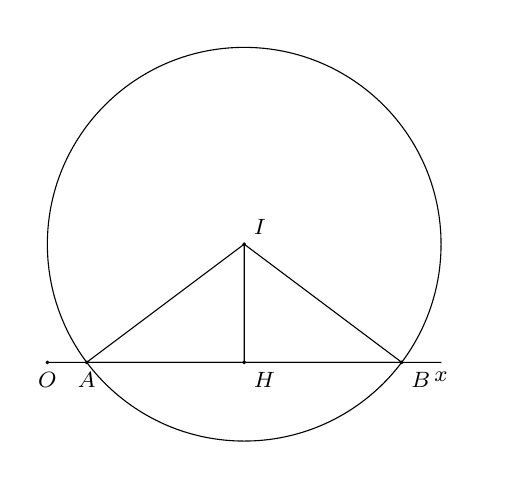
\begin{tikzpicture}[line join = round, line cap=round,>=stealth,font=\footnotesize,scale=0.5]
	\clip (-5.5,-5.5) rectangle (6,5.5);
	\def\r{5};
	\def\g{120};
	\def\gC{30};
	\path
	(0,0) coordinate (I)
	(-4,-3) coordinate (A)
	(4,-3) coordinate (B)
	(0,-3) coordinate (H)
	(-5,-3) coordinate (O);
	\draw (I) circle (\r);
	\draw(A)node[below]{$A$}circle(1pt)--(B)node[below right]{$B$}circle(1pt)--(I)node[above right]{$I$}circle(1pt)--(A)--(H)node[below right]{$H$}circle(1pt)--(I);
	\draw [->](O)node[below]{$O$}circle(1pt)--(5,-3)node[below]{$x$};
\end{tikzpicture}}
	}
\end{ex}

\begin{ex}%[Thi thử tốt nghiệp - THPT Yên Lạc 2-Vĩnh Phúc-23]%[Nguyễn Thành Nhân- EX6]%[2D3B2-1]
	Cho hàm số $f(x)$ có đạo hàm trên đoạn $\left[1;2023\right]$, $f(1)=1$, $f(2023)=2$. Tích phân $I=\displaystyle\int\limits_1^{2023} f'(x)\mathrm{\,d}x$ bằng
	\choice
	{$2022$}
	{\True $1$}
	{$2023$}
	{$2$}
	\loigiai{
	Ta có $I=\displaystyle\int\limits_1^{2023} f'(x)\mathrm{\,d}x=f(x)\bigg|_1^{2023}=f(2023)-f(1)=1$.
	}
\end{ex}
\begin{ex}%[Thi thử tốt nghiệp - THPT Yên Lạc 2-Vĩnh Phúc-23]%[Nguyễn Thành Nhân- EX6]%[2D1B2-4]
	Có bao nhiêu giá trị nguyên của $m$ thuộc $\left[-5;5\right]$ để hàm số $y=x^3-2x^2+(m+3)x-1$ không có cực trị?
	\choice
	{$6$}
	{$8$}
	{$5$}
	{\True $7$}
	\loigiai{
	Ta có $y'=3x^2-4x+m+3$ và $\Delta'=-3m-5$.\\
	Để hàm số không có cực trị thì $y'$ không đổi dấu trên $\mathbb{R}$, suy ra \[\Delta'\le 0\Leftrightarrow -3m-5\le 0\Leftrightarrow m\geq -\dfrac{5}{3}.\]
	Vì $m$ nguyên và $m\in \left[-5;5\right]$ nên $m\in \left\{-1;0;1;2;3;4;5\right\}$. Có $7$ giá trị.
	}
\end{ex}
\begin{ex}%[Thi thử tốt nghiệp - THPT Yên Lạc 2-Vĩnh Phúc-23]%[Nguyễn Thành Nhân- EX6]%[2H3B2-6]
	Trong không gian $Oxyz$, khoảng cách giữa hai mặt phẳng $\left(P\right)\colon x+2y+2z-10=0$ và $\left(Q\right)\colon x+2y+2z-5=0$ là 
	\choice
	{\True $\dfrac{5}{3}$}
	{$\dfrac{7}{3}$}
	{$5$}
	{$\dfrac{5}{9}$}
	\loigiai{
	Vì  $\dfrac{1}{1}=\dfrac{2}{2}=\dfrac{2}{2}\ne \dfrac{-10}{-5}$ nên $(P)\parallel (Q)$. Lấy điểm $A(0;0;5)$ thuộc $(P)$. Khi đó
	\[\mathrm{d}\left((P),(Q)\right)=\mathrm{d}\left(A,(Q)\right)=\dfrac{|0+0+10-5|}{\sqrt{1^2+2^2+2^2}}=\dfrac{5}{3}.\]
	}
\end{ex}



\begin{ex}%[Thi thử tốt nghiệp - THPT Yên Lạc 2-Vĩnh Phúc-23]%[Nguyễn Thành Nhân- EX6]%[2D1B4-3]
	Cho hàm số $y=f(x)$ xác định và có đạo hàm trên $\mathbb{R}\backslash \left\{-2;1\right\}$ và có bảng biến thiên như sau
	\begin{center}

\begin{tikzpicture}[>=stealth]
\tkzTabInit[nocadre=false,lgt=1.25,espcl=4,deltacl=0.5]
{$x$/0.75, $y'$/0.75, $y$/3}
{$-\infty$, $-2$, $1$, $+\infty$}
\tkzTabLine{,-,d,-,d,+,}
\tkzTabVar{+/$4$, -D+/$1$/$+\infty$, -D-/$2$/$2$, +/$+\infty$}
\end{tikzpicture}
\end{center}
	Đồ thị của hàm số có mấy đường tiệm cận?
	\choice
	{$0$}
	{$1$}
	{$3$}
	{\True $2$}
	\loigiai{
	Từ bảng biến thiên ta thấy\\
	$\lim\limits_{x\to -\infty }y=4$ nên đồ thị hàm số có đường tiệm cận ngang $y=4$.\\
	$\lim\limits_{x\to (-2)^+ }y=+\infty$ nên đồ thị hàm số có đường tiệm cận đứng $x=-2$.\\
	Vậy đồ thị hàm số có đường tiệm cận ngang $y=4$ và đường tiệm cận đứng $x=-2$.
	}
\end{ex}

\begin{ex}%[Thi thử tốt nghiệp - THPT Yên Lạc 2-Vĩnh Phúc-23]%[Nguyễn Thành Nhân- EX6]%[2H3Y2-2]
Trong không gian $Oxyz$, cho mặt phẳng $(P)\colon x-y+2z-3=0$. Một véc-tơ pháp tuyến của $(P)$ là 
	\choice
	{$\overrightarrow{n}=(1;1;-2)$}
	{\True $\overrightarrow{n}=(1;-1;2)$}
	{$\overrightarrow{n}=(1;2;-3)$}
	{$\overrightarrow{n}=(-1;2;-3)$}
	\loigiai{
	 Một véc-tơ pháp tuyến của $(P)$ là $\overrightarrow{n}=(1;-1;2)$.
	}
\end{ex}
\begin{ex}%[Thi thử tốt nghiệp - THPT Yên Lạc 2-Vĩnh Phúc-23]%[Nguyễn Thành Nhân- EX6]%[2D2B5-1]
Tổng các nghiệm của phương trình $\log_{2023}\left(x^2+2022x\right)=1$ bằng
	\choice
	{\True $-2022$}
	{$-2023$}
	{$2023$}
	{$2022$}
	\loigiai{
	 Ta có 
	 \begin{eqnarray*}
	 && \log_{2023}\left(x^2+2022x\right)=1 \Leftrightarrow x^2+2022x=2023\\
	 &\Leftrightarrow & x^2+2022x-2023=0\Leftrightarrow \hoac{&x=1\\&x=-2023.}
	 \end{eqnarray*}
	 Tổng các nghiệm $S=1+(-2023)=-2022$.
	}
\end{ex}

\begin{ex}%[Thi thử tốt nghiệp - THPT Yên Lạc 2-Vĩnh Phúc-23]%[Nguyễn Thành Nhân- EX6]%[1D3Y3-1]
Cho cấp số cộng $\left(u_n\right)$ có số hạng tổng quát $u_n=3n-2$ với $n\geq 1$. Công sai của cấp số cộng đã cho bằng
	\choice
	{$-2$}
	{$1$}
	{\True $3$}
	{$2$}
	\loigiai{
Từ công thức số hạng tổng quát ta có $u_1=1$; $u_2=4$. Do đó công sai $d=u_2-u_1=3$.
	}
\end{ex}



\begin{ex}%[Thi thử tốt nghiệp - THPT Yên Lạc 2-Vĩnh Phúc-23]%[Nguyễn Thành Nhân- EX6]%[2H1B3-2]
Cho hình chóp $S.ABCD$ có đáy $ABCD$ là hình chữ nhật, $AD=2AB$, $AC=\sqrt{5}$. $SA$ vuông góc với đáy và $SA=6$. Thể tích khối chóp đã cho bằng
	\choice
	{\True $4$}
	{$12$}
	{$6$}
	{$2$}
	\loigiai{
	\immini{
Đặt $AB=x$, $x>0$, suy ra $AD=2x$.\\
 Áp dụng định lý Py-ta-go cho tam giác vuông $ABD$ vuông tại $A$, ta có $x^2+2x^2=5\Leftrightarrow x=1$.\\
Diện tích hình chữ nhật $ABCD$ là $S=AB\cdot CD=2\cdot 1=2$. Thể tích khối chóp là
\[V_{S.ABCD}=\dfrac{1}{3}\cdot SA\cdot S_{ABCD}=\dfrac{1}{3}\cdot 6\cdot 2=4.\]}
{\begin{tikzpicture}[line join = round, line cap=round,>=stealth,font=\footnotesize,scale=0.5]
	\clip (-4,-4) rectangle (9,7);
	\def\r{5};
	\def\g{120};
	\def\gC{30};
	\path
	(0,0) coordinate (A)
	(-3,-3) coordinate (B)
	(5,-3) coordinate (C)
	(8,0) coordinate (D)
	(0,6) coordinate (S);
	\draw(B)node[below left]{$B$}circle(1pt)--(C)node[below right]{$C$}circle(1pt)--(D)node[above right]{$D$}circle(1pt)--(S)--(C)--(S)--(B);
	\draw[dashed](B)--(A)node[above left]{$A$}circle(1pt)--(S)node[above left]{$S$}circle(1pt);
	\draw[dashed](D)--(A);
\end{tikzpicture}}
	}
\end{ex}

\begin{ex}%[Thi thử tốt nghiệp - THPT Yên Lạc 2-Vĩnh Phúc-23]%[Nguyễn Thành Nhân- EX6]%[2D2B2-1]
Tập xác định của hàm số $y=\left(1+x\right)^{-2023}$ là
	\choice
	{$(-1;+\infty)$}
	{\True $\mathrm{R}\backslash \left\{-1\right\}$}
	{$(-\infty;-1)$}
	{$\mathrm{R}\backslash \left\{0\right\}$}
	\loigiai{
	Điều kiện xác định $x+1\ne 0\Leftrightarrow x\ne -1$.\\
	Vậy tập xác định của hàm số là $\mathrm{R}\backslash \left\{-1\right\}$. 
	}
\end{ex}
\begin{ex}%[Thi thử tốt nghiệp - THPT Yên Lạc 2-Vĩnh Phúc-23]%[Nguyễn Thành Nhân- EX6]%[2D2K4-1]
Có tất cả bao nhiêu giá trị nguyên của tham số $m\in (-2023;2023)$ để hàm số $y=\dfrac{2023}{m\log_3^2x-4\log_3x+m+3}$ xác định trên khoảng $(0;+\infty)$.
	\choice
	{$4040$}
	{$4044$}
	{\True $4039$}
	{$4046$}
	\loigiai{
	Đặt $t=\log_3x$. Với $x\in (0;+\infty)$ thì $t\in \mathbb{R}$. Hàm số trở thành $y=\dfrac{2023}{mt^2-4t+m+3}$.\\
	Để hàm số đã cho xác định trên khoảng $(0;+\infty)$ thì hàm số  $y=\dfrac{2023}{mt^2-4t+m+3}$ phải xác định với mọi $t\in \mathbb{R}$.\\
	Đặt $g(t)=mt^2-4t+m+3$.\\
	 Với $m=0$ thì $g(t)=-4t+3\ne 0$ khi $t\ne \dfrac{3}{4}$ nên loại $m=0$.\\
	 Với $m\ne 0$. Để hàm số xác định với mọi $t$ thì phương trình $g(t)=0$ vô nghiệm
	 \[\Leftrightarrow \Delta <0\Leftrightarrow 4-m^2-3m<0\Leftrightarrow \hoac{&m<-4\\&m>1.}\]
	 Đối chiếu với giả thiết bài toán ta được $m\in \left\{-2022;-2021;\ldots;-5\right\}\cup \left\{2;3;2022\right\}$.\\
	 Có tất cả $4039$ giá trị nguyên $m$.
	}
\end{ex}
\begin{ex}%[Thi thử tốt nghiệp - THPT Yên Lạc 2-Vĩnh Phúc-23]%[Nguyễn Thành Nhân- EX6]%[2H2K2-2]
	Cho tứ diện $ABCD$ có các mặt $ABC$, $BCD$ là tam giác đều cạnh bằng $2$, hai mặt $(ABD)$ và $(ACD)$ vuông góc với nhau. Bán kính mặt cầu ngoại tiếp tứ diện $ABCD$ bằng 
	\choice
	{$\dfrac{2\sqrt{2}}{3}$}
	{\True $\sqrt{2}$}
	{$2\sqrt{2}$}
	{$\dfrac{\sqrt{6}}{3}$}
	\loigiai{
	\immini{Từ giả thiết các tam giác  $ABC$, $BCD$ đều cạnh $2$ suy ra $CA=CD=2$, $BA=BD=2$ nên các tam giác $CAD$ và $BAD$ lần lượt cân tại $C$ và $B$.\\
	Gọi $H$ là trung điểm $AD$, suy ra $CH\perp AD$. Vì $(BAD)\perp ( ACD)$ nên suy ra $CH\perp (ABD)$. Suy ra $CH\perp BH$.\\
	Lại có $\triangle BAD=\triangle CAD$ nên $BH=CH$. Từ đó suy ra ta giác $BHC$ vuông cân tại $H$ có cạnh huyền $BC=2\Rightarrow BH=CH=\sqrt{2}$.\\
	Tam giác $CAH$ vuông tại $H$ có $\cos\widehat{ACH}=\dfrac{CH}{AC}=\dfrac{\sqrt{2}}{2}\Rightarrow \widehat{ACH}=45^{\circ}$.
	}
	{\begin{tikzpicture}[line join = round, line cap=round,>=stealth,font=\footnotesize,scale=0.4]
	\clip (-1,-4) rectangle (13,7);
	\def\r{5};
	\def\g{120};
	\def\gC{30};
	\path
	(0,0) coordinate (A)
	(3,6) coordinate (C)
	(12,0) coordinate (B)
	(5,-3) coordinate (D);
	\coordinate (H) at ($(A)!.5!(D)$);
	\draw(A)node[below left]{$A$}circle(1pt)--(D)node[below right]{$D$}circle(1pt)--(B)node[above right]{$B$}circle(1pt)--(C)node[above right]{$C$}circle(1pt)--(H)node[below left]{$H$}circle(1pt)--(A)--(D)--(C)--(A);
	\draw[dashed](A)--(B)--(H);
\end{tikzpicture}}
Tam giác $ACD$ cân tại $C$ nên $CH$ là đường phân giác, do đó $\widehat{ACD}
	=90^{\circ}$. Tam giác $ACD$ vuông cân tại $C$. Suy ra $CH=AH=DH.\quad (1)$. \\
	Lại có $\triangle CAD=\triangle BAD\,(c-c-c)$ nên $\triangle BAD$ vuông cân tại $B$. Suy ra $BH=AH=DH.\quad (2)$	\\
	Từ $(1)$ và $(2)$ suy ra $HA=HB=HC=HD=\sqrt{2}$, do đó $H$ là tâm mặt cầu ngoại tiếp tứ diện $ABCD$ bán kính bằng $\sqrt{2}$.
	}
\end{ex}
\begin{ex}%[Thi thử tốt nghiệp - THPT Yên Lạc 2-Vĩnh Phúc-23]%[Nguyễn Thành Nhân- EX6]%[1H3K5-3]
	Cho hình chóp $S.ABCD$ có đáy $ABCD$ là hình vuông tâm $O$, $SA=2a\sqrt{2}$. Hình chiếu vuông góc của $S$ lên mặt phẳng $(ABCD)$ trùng với trung điểm của cạnh $OA$, biết tam giác $SBD$ vuông tại $S$. Khoảng cách từ $D$ đến mặt phẳng $(SBC)$ bằng
	\choice
	{$\dfrac{3a\sqrt{5}}{10}$}
	{$\dfrac{2a\sqrt{5}}{5}$}
	{\True $\dfrac{4a\sqrt{10}}{5}$}
	{$\dfrac{2a\sqrt{10}}{5}$}
	\loigiai{
	\immini{Gọi $H$ là hình chiếu của $S$ lên $(ABCD)$ thì $H$ là trung điểm của $OA$.\\
	Vì $AD\parallel BC$ nên $AD\parallel (SBC)$ và $\dfrac{AC}{HC}=\dfrac{4}{3}$. Do đó
	\[\mathrm{d}\left(D,(SBC)\right)=\mathrm{d}\left(A,(SBC)\right)=\dfrac{AC}{HC}\cdot\mathrm{d}\left(H,(SBC)\right)=\dfrac{4}{3}\mathrm{d}\left(H,(SBC)\right).\]
	Kẻ $HK\perp BC$, suy ra $BC\perp (SHK)\Rightarrow (SBC)\perp (SHK)$.\\
	Kẻ $HE\perp SK$ thì $HE\perp (SBC)$ nên $HE=\mathrm{d}\left(H,(SBC)\right)$.\\
	$\triangle SHK$ vuông tại $H$ có $HE$ là đường cao nên
	\[HE=\dfrac{SH\cdot HK}{\sqrt{SH^2+HK^2}}.\quad (*)\]
	}
	{\begin{tikzpicture}[line join = round, line cap=round,>=stealth,font=\footnotesize,scale=0.6]
	\clip (-3,-5) rectangle (9,6);
	\def\r{5};
	\def\g{120};
	\def\gC{30};
	\path
	(0,0) coordinate (A)
	(-2,-4) coordinate (B)
	(6,-4) coordinate (C)
	(8,0) coordinate (D)
	(1.5,5) coordinate (S)
	(1.5,-1)coordinate (H)
	(0,-4)coordinate (K)
	(3,-2)coordinate (O);
	\coordinate (E) at ($(S)!.5!(K)$);
	\draw(B)node[below left]{$B$}circle(1pt)--(C)node[below right]{$C$}circle(1pt)--(D)node[above right]{$D$}circle(1pt)--(S)node[above right]{$S$}circle(1pt)--(B)--(C)--(S)--(K);
	\draw[dashed](A)node[below]{$A$}circle(1pt)--(B)--(D);
	\draw[dashed](C)--(O)node[above right]{$O$}circle(1pt)--(S)--(H)node[below left]{$H$}circle(1pt);
	\draw[dashed](A)--(S)--(O)--(D)--(H)--(K)node[below left]{$K$}circle(1pt)--(H)--(E)node[above right]{$E$}circle(1pt);
	\draw[dashed](A)--(D);
	\draw[dashed](O)--(A);
\end{tikzpicture}
	}
	Tam giác $SBD$ vuông tại $S$ nên $SO=\dfrac{1}{2}BD=\dfrac{1}{2}AC$, suy ra tam giác $SAC$ vuông tại $S$. Do đó
	\[AH\cdot AC=AS^2\Leftrightarrow 4AH^2=AS^2\Leftrightarrow AH=\dfrac{AS}{2}=a\sqrt{2}.\]
	Do đó $AC=4AH=4a\sqrt{2}\Leftrightarrow AB=4a$ và $SH=\sqrt{SA^2-AH^2}=a\sqrt{6}$.\\
	Ta có $\dfrac{HK}{AB}=\dfrac{CH}{CA}=\dfrac{3}{4}\Leftrightarrow HK=\dfrac{3}{4}AB=3a$.\\
	Thay vào $(*)$ ta được
	\[HE=\dfrac{a\sqrt{6}\cdot 3a}{a\sqrt{15}}=\dfrac{3a\sqrt{10}}{5}.\]
	Vậy $\mathrm{d}\left(D,(SBC)\right)=\dfrac{4}{3}HE=\dfrac{4a\sqrt{10}}{5}$.
	}
\end{ex}
\begin{ex}%[Đề thi thử THPT Yên Lạc 2 Vĩnh Phúc]%[Nguyễn Thành Nhân, 12EX-5-2223]%[2D3K3-3] 
	Khối tròn xoay tạo thành khi quay hình phẳng $ (H) $ giới hạn bởi đường cong $ y=\sqrt{\dfrac{5+(x-4)\mathrm{e}^x}{x\mathrm{e}^x+1}} $, trục hoành và hai đường thẳng $ x=0 $, $ x=1 $ quanh trục hoành có thể tích $ V=\pi[a+b\ln(e+1)] $, trong đó $ a $, $ b $ là các số nguyên. Mệnh đề nào dưới đây đúng?
	\choice
	{$ a+b=9 $}
	{$ a+b=5 $}
	{\True $ 2a-b=14 $}
	{$ a-2b=-3 $}
	\loigiai{
		Thể tích khối tròn xoay khi quay hình phẳng $ (H) $ là 
		\begin{eqnarray*}
			V=\pi \displaystyle\int\limits_{0}^{1} \dfrac{5+(x-4)\mathrm{e}^x}{x\mathrm{e}^x+1} \mathrm{\,d}x&= & \pi \displaystyle\int\limits_{0}^{1}\dfrac{5(1+x\mathrm{e}^x)-4\mathrm{e}^x(x+1)}{x\mathrm{e}^x+1} \mathrm{\,d}x\\
			&= & \pi \displaystyle\int\limits_{0}^{1}\left(5-\dfrac{4\mathrm{e}^x(x+1)}{x\mathrm{e}^x+1} \right)  \mathrm{\,d}x\\
			&= &\pi\displaystyle\int\limits_{0}^{1} 5\mathrm{\,d}x-4\pi \displaystyle\int\limits_{0}^{1}\dfrac{1}{x\mathrm{e}^x+1} \mathrm{\,d}(x\mathrm{e}^x+1)\\
			&=&5\pi -4\pi \left( \ln|x\mathrm{e}^x+1|\right)\bigg|_0^1=\pi (5-4\ln(\mathrm{e}+1)).
		\end{eqnarray*}
	Khi đó $ a=5 $, $ b=-4 $ suy ra $ 2a-b=14 $.
	}
\end{ex}

\begin{ex}%[Đề thi thử THPT Yên Lạc 2 Vĩnh Phúc]%[Nguyễn Thành Nhân, 12EX-5-2223]%[2D1K5-4]
	Cho hàm số $ y=\dfrac{2x+1}{x+1}  $ có đồ thị $ (C) $. Có bao nhiêu giá trị của $ m $ để đường thẳng $ d\colon y=-2x+m $ cắt $ (C) $ tại hai điểm phân biệt $ A $, $ B $ sao cho tam giác $ OAB $ có diện tích bằng $ \sqrt{3} $?
	\choice
	{\True $ 2 $}
	{$ 0 $}
	{$ 3 $}
	{$ 1 $}
	\loigiai{
	Xét phương trình hoành độ giao điểm của $ (C) $ và $ d $.
	\begin{eqnarray*}
		& &-2x+m= \dfrac{2x+1}{x+1} \\
		&\Leftrightarrow & 2x^2-(m-4)x+1-m=0~(*)\quad(x \ne -1)\\
	\end{eqnarray*}
Do $\heva{&\Delta =m^2+8>0 \\& 2(-1)^2-(m-4)(-1)+1-m \ne 0} $ nên $(*)$ luôn có hai nghiệm phân biệt $x_1$, $x_2$ khác $-1$. \\
Gọi $A(x_1;-2x_1+m)$, $B(x_2;-2x_2+m)$ là các giao điểm của đồ thị hai hàm số trên. Ta có
\begin{eqnarray*}
	AB=\sqrt{{(x_2-x_1)}^2+{(2x_1-2x_2)}^2}& =&\sqrt{5\left[{(x_1+x_2)}^2-4x_1x_2\right]} \\
	&=& \sqrt{5\left[{\left(\dfrac{m-4}{2}\right)}^2-4\cdot \left(\dfrac{1-m}{2}\right)\right]}\\
	&= & \sqrt{\dfrac{5(m^2+8)}{4}}.
\end{eqnarray*}
Do $AB\colon y=-2x+m \Leftrightarrow 2x+y-m=0$ nên $ \mathrm{\,d}(O,AB)=\dfrac{|m|}{\sqrt{5}}$.\\
$S_{\triangle OAB}=\dfrac{1}{2}AB\cdot \mathrm{\,d}(O,AB)=\sqrt{3} \Leftrightarrow \dfrac{|m|}{2}\sqrt{\dfrac{m^2+8}{4}}=\sqrt{3} \Leftrightarrow \dfrac{m^2(m^2+8)}{16}=3 \Leftrightarrow m^2=4$.\\
Với $m^2=4$ suy ra $m=2$ hoặc $m=-2$ thỏa mãn yêu cầu đề bài.
	}
\end{ex}

\begin{ex}%[Đề thi thử THPT Yên Lạc 2 Vĩnh Phúc]%[Nguyễn Thành Nhân, 12EX-5-2223]%[1H3K2-3]
	Cho hình chóp $ S.ABCD $ có đáy là hình vuông cạnh $ 2a $, $ SA\perp (ABCD) $ và $ SB=a\sqrt{5} $. Gọi $ M $ là trung điểm của $ AB $ và $ N $ là trung điểm của $ AD $. Tính cosin góc giữa hai đường thẳng $ SM $ và $ BN $.
	\choice
	{\True $ \dfrac{\sqrt{10}}{5} $}
	{$ \dfrac{1}{\sqrt{10}} $}
	{$ \dfrac{2\sqrt{5}}{5} $}
	{$ \dfrac{5}{5} $}
	\loigiai{
		\immini{
			Gọi $ K $ là trung điểm của $ AN $ suy ra $ MK\parallel BN $.\\
			Khi đó góc giữa hai đường thẳng $ SM $ và $ BN $ bằng góc giữa hai đường thẳng $ SM $ và $ MK $ bằng $ \widehat{SMK} $.\\
			Ta có $ MK $ là đường trung bình trong $ \triangle ABN $ suy ra $$ MK=\dfrac{BN}{2}=\dfrac{\sqrt{AB^2+AN^2}}{2}=\dfrac{\sqrt{(2a)^2+a^2}}{2}=\dfrac{a\sqrt{5}}{2}. $$
			Ta có $ SA=\sqrt{SB^2-AB^2}=\sqrt{(a\sqrt{5})^2-(2a)^2}=a $.\\
			Lại có $ SM=\sqrt{SA^2+AM^2}=\sqrt{a^2+a^2}=a\sqrt{2} $.\\
			Ta có $ SK=\sqrt{SA^2+AK^2}=\sqrt{a^2+\dfrac{a^2}{4}}=\dfrac{a\sqrt{5}}{2} $.
		}{\begin{tikzpicture}[line cap=round, line join=round, font=\footnotesize, >=stealth, scale=0.7]
		\tikzset{label style/.style={font=\footnotesize}}
		\def\s{2}
		\path (0,0) coordinate (A)circle(1pt)
		(-1.5,-1) coordinate (B)circle(1pt)
		(3,0) coordinate (D)circle(1pt)
		($(D)+(B)-(A)$) coordinate (C)circle(1pt)
		($(A)+(0,\s)$) coordinate (S)circle(1pt)
		($(B)!0.5!(A)$) coordinate (M)circle(1pt)
		($(D)!0.5!(A)$) coordinate (N)circle(1pt)
		($(A)!0.5!(N)$) coordinate (K)circle(1pt);
		\draw (S)--(B)--(C)--(D)--(S)--(C);
		\draw[dashed] (S)--(A)--(B) (K)--(M)--(S)--(K) (B)--(N) (A)--(D);
		\foreach \x/\y in {S/90, A/150, B/-135, C/-45, D/0,M/120, K/145, N/30} \draw[fill=black] (\x) circle (1pt) +(\y:0.3) node{$\x$};
		\end{tikzpicture}}
	Do đó $ \cos\widehat{SMK}=\dfrac{SM^2+MK^2-SK^2}{2SM\cdot MK}=\dfrac{(a\sqrt{2})^2+\left(\dfrac{a\sqrt{5}}{2} \right)^2-\left(\dfrac{a\sqrt{5}}{2} \right)^2 }{2\cdot a\sqrt{2}\cdot\dfrac{a\sqrt{5}}{2} }=\dfrac{\sqrt{10}}{5} $.
	}
\end{ex}
\begin{ex}%[Thi thử tốt nghiệp - THPT Yên Lạc 2-Vĩnh Phúc-23]%[Nguyễn Thành Nhân- EX6]%[2D1K1-2]
\immini{
Cho hàm số bậc ba $y=f(x)=ax^3+bx^2+cx+d$ có đồ thị $\left(\mathscr{C}\right)$ và hàm số $y=g(x)=-f\left(mx+1\right)$, $m>0$ (như hình vẽ). Với giá trị nào của $m$ thì hàm số $y=g(x)$ nghịch biến trên đúng một khoảng có độ dài bằng $3$?
	\choice
	{$\dfrac{2}{3}$}
	{$\dfrac{2}{5}$}
	{$\dfrac{1}{3}$}
	{\True $\dfrac{1}{2}$}}
	{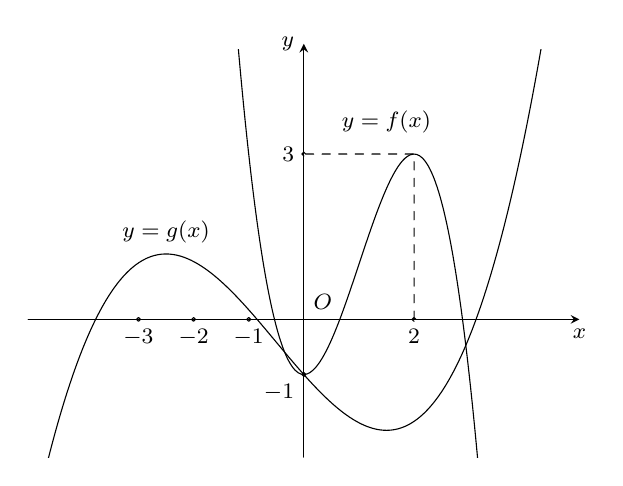
\begin{tikzpicture}[scale=0.7, font=\footnotesize,line join=round, line cap=round, >=stealth]
    \def\xt{-5} \def\xp{5} \def\yt{5} \def\yd{-2.5}
    \draw[->] (\xt,0)--(\xp,0) node [below]{$x$};
    \draw[->] (0,\yd)--(0,\yt) node [left]{$y$};
    \node at (0,0) [above right]{$O$};
    \clip (\xt,\yd) rectangle (\xp-0.1,\yt-0.1);
    \draw[smooth,samples=150,domain=-3:5] plot(\x,{-1*(\x)^3+3*(\x)^2-1});
     \draw[smooth,samples=150,domain=-5:5] plot(\x,{0.1*(\x)^3+0.15*(\x)^2-1.125*(\x)-1});
    \draw[dashed] (2,0)node[below]{$2$}circle(1pt)|-(2,3)--(0,3)node[left]{$3$}circle(1pt);
    \draw(-2,0)node[below]{$-2$}circle(1pt)(-1,0)node[below]{$-1$}circle(1pt)(-3,0)node[below]{$-3$}circle(1pt)(0,-1)node[below left]{$-1$}circle(1pt);
    \draw(-2.5,1.2)node[above]{$y=g(x)$}(1.5,3.2)node[above]{$y=f(x)$};
    \fill[black](-2,0)(-1,0)(-3,0)(0,-1)(2,0)(2,3)(0,3);
    \end{tikzpicture}}
	\loigiai{
Từ đồ thị hàm số $y=f(x)$, ta suy ra hàm số $f(x)$ có hai cực trị $x=0$ và $x=2$. Do đó $f'(x)=3ax^2+2bx+c$ có hai nghiệm $x=0$, $x=2$.\\
Đồ thị hàm số có hai điểm cực trị là $(0,-1)$ và $(2,3)$ nên ta có $f(0)=-1$ và $f(2)=3$. Ta có hệ phương trình
\[\heva{&f'(0)=0\\&f'(2)=0\\&f(2)=3\\&f(0)=-1}\Leftrightarrow \heva{&c=0\\&12a+4b+c=0\\&8a+4b+2c+d=3\\&d=-1}\Leftrightarrow \heva{&a=-1\\&b=3\\&c=0\\&d=-1.}\]
Ta có $y=f(x)=-x^3+3x^2-1$.\\
Xét hàm số $y=g(x)=-f\left(mx+1\right)$. Ta có $g'(x)=-mf'\left(mx+1\right)$.\\
Hàm số nghịch biến 
\begin{eqnarray*}
g'(x)\le 0\Leftrightarrow  f'\left(mx+1\right)\geq 0\Leftrightarrow 0\le mx+1\le 2\Leftrightarrow -\dfrac{1}{m}\le x\le \dfrac{1}{m}.
\end{eqnarray*}
Do đó hàm số $y=g(x)$ nghịch biến trên đoạn $\left[ -\dfrac{1}{m}; \dfrac{1}{m}\right]$.\\
Hàm số nghịch biến trên một đoạn có độ dài bằng $3$ nên 
\[\dfrac{1}{m}-\left( -\dfrac{1}{m}\right)=3\Leftrightarrow \dfrac{2}{m}=3\Leftrightarrow m=\dfrac{2}{3}.\]
	}
\end{ex}

\begin{ex}%[Thi thử tốt nghiệp - THPT Yên Lạc 2-Vĩnh Phúc-23]%[Nguyễn Thành Nhân- EX6]%[2H3K3-1]
Trong không gian $Oxyz$, cho hình lăng trụ tam giác đều $ABC.A'B'C'$ có $A'(\sqrt{3};-1;1)$, hai đỉnh $B$, $C$ thuộc trục $Oz$ và $AA'=1$ ($C$ không trùng với $O$). Biết véc-tơ $\overrightarrow{u}=(a;b;2)$ với $a$, $b\in \mathbb{R}$ là một véc-tơ chỉ phương của đường thẳng $A'C$. Tính $T=a^2+b^2$.
	\choice
	{$T=5$}
	{$T=14$}
	{\True $T=16$}
	{$T=9$}
	\loigiai{
\immini{Gọi $M$ là trung điểm $BC$. Khi đó \[\heva{&BC\perp AM\\&BC\perp AA'}\Leftrightarrow BC\perp (AMA')\Rightarrow BC\perp A'M.\]
Do đó $M$ là hình chiếu của $A'$ lên $BC$, tức là lên trục $Oz$, suy ra $M(0;0;1)$ và $A'M=2$. Ta có
$AM=\sqrt{A'M^2-AA'^2}=\sqrt{3}$. Tam giác $ABC$ đều nên $BC=2\Rightarrow MB=MC=1$. Vì $C\in Oz$ và $C\not \equiv O$ nên $C(0;0;c)$ với $c\ne 0$. Ta có
\begin{eqnarray*}
&& MC=1\Leftrightarrow |c-1|=1\Leftrightarrow \hoac{&c=2\\&c=0}\Rightarrow c=2\Rightarrow C(0;0;2).
\end{eqnarray*}
Ta có $\overrightarrow{A'C}=(-\sqrt{3};1;1)$ là một véc-tơ chỉ phương của đường thẳng $A'C$. Do đó $\overrightarrow{u}=(-2\sqrt{3};2;2)$ cũng là một véc-tơ chỉ phương của đường thẳng $A'C$. Do đó $a=-2\sqrt{2}$, $b=2$. \\
Vậy $T=a^2+b^2=16$.
}
{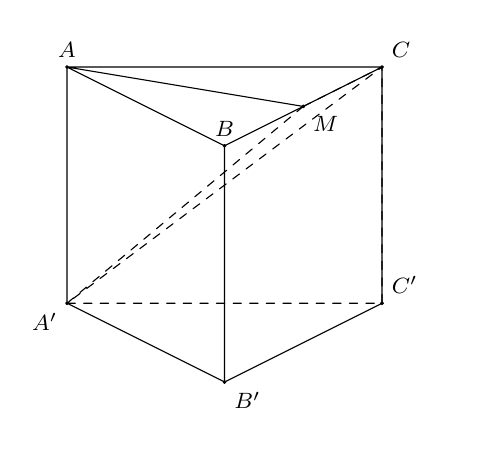
\begin{tikzpicture}[line join = round, line cap=round,>=stealth,font=\footnotesize,scale=0.5]
	\clip (-1,-3) rectangle (10,7);
	\def\r{5};
	\def\g{120};
	\def\gC{30};
	\path
	(0,6) coordinate (A)
	(4,4) coordinate (B)
	(8,6) coordinate (C)
	(0,0) coordinate (A')
	(4,-2) coordinate (B')
	(8,0) coordinate (C')
	(6,5) coordinate (M);
	\draw(A)node[above]{$A$}circle(1pt)--(B)node[above]{$B$}circle(1pt)--(C)node[above right]{$C$}circle(1pt)--(C')node[above right]{$C'$}circle(1pt)--(B')node[below right]{$B'$}circle(1pt)--(A')node[below left]{$A'$}circle(1pt)--(A)--(C)--(B)--(B')--(B)--(M)--(A);
	\draw[dashed](A')--(C')--(C)--(M)node[below right]{$M$}circle(1pt)--(A')--(C);
\end{tikzpicture}
}
	}
\end{ex}
\begin{ex}%[Thi thử tốt nghiệp - THPT Yên Lạc 2-Vĩnh Phúc-23]%[Nguyễn Thành Nhân- EX6]%[2D2K5-3]
	Số nghiệm của phương trình $\log_3\left|x^2-\sqrt{2}x\right|=\log_5\left(x^2-\sqrt{2}x+2\right)$ là
	\choice
	{\True $2$}
	{$0$}
	{$1$}
	{$3$}
	\loigiai{Điều kiện $\heva{&x^2-\sqrt{2}x\ne 0\\&x^2-\sqrt{2}x+2>0}\Leftrightarrow \heva{&x\ne 0\\&x\ne \sqrt{2}\\&\forall x\in \mathbb{R}}\Leftrightarrow \heva{&x\ne 0\\&x\ne \sqrt{2}.}$\\
Đặt $\log_3\left|x^2-\sqrt{2}x\right|=\log_5\left(x^2-\sqrt{2}x+2\right)=t$. Khi đó $\heva{&\left|x^2-\sqrt{2}x\right|=3^t\\&x^2-\sqrt{2}x=5^t-2}$. Do đó ta có phương trình
\begin{eqnarray*}
&& \left|5^t-2\right|=3^t\Leftrightarrow \hoac{&5^t-2=3^t\\&5^t-2=-3^t}\Leftrightarrow \hoac{&\left(\dfrac{3}{5}\right)^t+2\cdot \left(\dfrac{1}{5}\right)^t=1\quad (1)\\&5^t+3^t=2.\quad (2)}
\end{eqnarray*}
	Xét phương trình $(1)$, đặt $f(t)=\left(\dfrac{3}{5}\right)^t+2\cdot \left(\dfrac{1}{5}\right)^t$ có $f'(t)=\left(\dfrac{3}{5}\right)^t\cdot \ln \dfrac{3}{5}+2\left(\dfrac{1}{5}\right)^t\cdot \ln \dfrac{1}{5}<0,\,\forall t$ nên $f(t)$ nghịch biến. Trong khi vế phải là hàm hằng. Do đó nếu $(1)$ có nghiệm thì nghiệm đó là duy nhất.\\
	Lại có $f(1)=1$ nên $t=1$ là nghiệm duy nhất của $(1)$.\\
	Với $t=1$ thì $x^2-\sqrt{2}x=3\Leftrightarrow x^2-\sqrt{2}x-3=0$. Phương trình này có hai nghiệm $x$.\\
	Xét phương trình $(2)$, đặt $g(t)=5^t+3^t$ thì $g'(t)=5^t\cdot \ln 5+3^t\cdot \ln 3>0,\,\forall t$. Do đó $g(t)$ nghịch biến, trong khi vế phải là hằng số. Nên nếu phương trình có nghiệm thì nghiệm là duy nhất. Lại có $g(0)=2$ nên $t=0$ là nghiệm duy nhất.\\
	Với $t=0$ thì $x^2-\sqrt{x}=-2\Leftrightarrow x^2-\sqrt{2}x+2=0$. Phương trình này vô nghiệm đối với $x$.\\
	Vậy phương trình đã cho có hai nghiệm.
	}
\end{ex}
\begin{ex}%[Thi thử tốt nghiệp - THPT Yên Lạc 2-Vĩnh Phúc-23]%[Nguyễn Thành Nhân- EX6]%[2D1K1-3]
	Gọi $S$ là tập tất cả các giá trị nguyên của tham số $m$ để hàm số $y=(m-3)x-(2m+1)\cos x$ luôn nghịch biến trên $\mathbb{R}$. Số phần tử của $S$ bằng
	\choice
	{$6$}
	{$7$}
	{\True $5$}
	{$4$}
	\loigiai{
	Ta có $y'=m-3+(2m+1)\sin x$,\\
	Để hàm số nghịch biến trên $\mathbb{R}$ thì 
	\begin{eqnarray*}
	&& y'\le 0,\,\forall x\in \mathbb{R}\\
	&\Leftrightarrow & m-3+(2m+1)\sin x\le 0,\,\forall x\in \mathbb{R}.
	\end{eqnarray*}
	Đặt $t=\sin x$ thì $t\in \left[-1;1\right]$. Bất phương trình trở thành $(2m+1)t+m-3\le 0$.\\
	Đặt $f(t)=  (2m+1)t+m-3$ với $t\in \left[-1;1\right]$.\\
	Để $f(t)\le 0,\,\forall t\in  \left[-1;1\right]$ thì 
	\[\max\limits_{\left[-1;1\right]}\left\{f(-1);f(1)\right\}\le 0\Leftrightarrow \heva{&-m-4\le 0\\&3m-2\le 0}\Leftrightarrow \heva{&m\geq -4\\&m\le \dfrac{2}{3}}\Leftrightarrow -4\le m\le \dfrac{2}{3}.\] 
	Vì $m\in \mathbb{Z}$ nên $m\in \left\{-4;-3;-2;-1;0\right\}$. \\
	Vậy có $5$ giá trị nguyên của $m$ thỏa mãn bài toán.
	}
\end{ex}
\begin{ex}%[Đề thi thử THPT Yên Lạc 2 Vĩnh Phúc]%[Nguyễn Thành Nhân, 12EX-5-2223]%[2H1K3-3]
	Cho hình chóp đều $ S.ABC $ có $ \widehat{ASB}=30^\circ $, $ SA=1 $. Lấy $ B' $, $ C' $ lần lượt thuộc cạnh $ SB $, $ SC $ sao cho chu vi tam giác $ AB'C' $ nhỏ nhất. Tỉ số $ \dfrac{V_{S.AB'C'}}{V_{S.ABC}} $ gần giá trị nào nhất trong các giá trị sau?
	\choice
	{$ 0{,}5 $}
	{$ 0{,}6 $}
	{\True $ 0{,}55 $}
	{$ 0{,65} $}
	\loigiai{\immini{	Trải các mặt bên của hình chóp lên mặt phẳng $ (SBC) $.\\
			Suy ra chu vi $ 	\triangle AB'C' $
			\begin{eqnarray*}
				C_{\triangle AB'C'}	& =& AB'+B'C'+AC'\\
				&= & AB'+B'C'+C'A_1\\
				&\ge  & AA_1.
			\end{eqnarray*} 
			Do đó chu vi nhỏ nhất của tam giác bằng $ AA_1 $.\\
			Ta có $ \widehat{ASA_1}=30^\circ+30^\circ+30^\circ=90^\circ $.\\
			Suy ra  $ \triangle ASA_1 $ vuông cân tại $ S $ suy ra $ AA_1=\sqrt{2} $.\\
			Từ đó suy ra chu vi nhỏ nhất bằng $ \sqrt{2} $.\\
			Dấu bằng xảy ra khi $ A $, $ B' $, $ C' $, $ A_1 $ thẳng hàng.\\
			Ta có $ \dfrac{SB'}{\sin SAB'}=\dfrac{SA}{\sin SB'A} $.\\
			Khi đó $ \dfrac{SB'}{SB}=\dfrac{\sin SAB'}{\sin SB'A}=\dfrac{\sin45^\circ}{\sin 105^\circ}=-1+\sqrt{3} $.\\
			Vậy $ \dfrac{V_{SAB'C'}}{V_{SABC}}=\dfrac{SB'}{SB}\cdot\dfrac{SC'}{SC}\cdot\dfrac{SA}{SA}=(-1+\sqrt{3})\cdot(-1+\sqrt{3})=4-2\sqrt{3}\approx 0{,}54 $.}{\begin{tikzpicture}[line cap=round, line join=round, font=\footnotesize, >=stealth, scale=1]
			\tikzset{label style/.style={font=\footnotesize}}
			\def\s{2}
			\path (0,1) coordinate (A)
			(1,-1) coordinate (B)
			(4,-1) coordinate (C)
			(2.5,3) coordinate (S)
			(5,1) coordinate (D)
			($(C)!0.5!(S)$) coordinate (C')
			($(B)!0.5!(S)$) coordinate (B');
			\draw (B)--(A)--(S)--(B)--(C)--(D)--(S)--(C) (A)--(D);
			\fill (D) node[right]{$A_1$} circle (1pt);
			\foreach \x/\y in {S/90, A/150, B/-135, C/-45, B'/120, C'/60} \draw[fill=black] (\x) circle (1pt) +(\y:0.3) node{$\x$};
			\end{tikzpicture}	}
	
	}
\end{ex}

\begin{ex}%[Thi thử tốt nghiệp - THPT Yên Lạc 2-Vĩnh Phúc-23]%[Nguyễn Thành Nhân- EX6]%[2D3K2-3]
	Cho hàm số $f(x)$ liên tục, có đạo hàm trên $\mathbb{R}$, $f(2)=16$, $\displaystyle\int\limits_0^{2} f(x)\mathrm{\,d}x=4$. Tích phân $\displaystyle\int\limits_0^{4} xf'\left(\dfrac{x}{2}\right)\mathrm{\,d}x$ bằng
	\choice
	{\True $112$}
	{$144$}
	{$56$}
	{$12$}
	\loigiai{
	Xét tích phân $I=\displaystyle\int\limits_0^{4} xf'\left(\dfrac{x}{2}\right)\mathrm{\,d}x$. \\
	Đặt $t=\dfrac{x}{2}\Rightarrow \mathrm{\,d}t=\dfrac{1}{2}\mathrm{\,d}x\Rightarrow \mathrm{\,d}x=2\mathrm{\,d}t$. Tích phân trở thành $I=4\displaystyle\int\limits_0^{2} tf'\left(t\right)\mathrm{\,d}t=4\displaystyle\int\limits_0^{2} xf'\left(x\right)\mathrm{\,d}x$.\\
	Đặt $\heva{&u=x\\&\mathrm{\,d}v=f'\left(x\right)\mathrm{\,d}x}\Rightarrow \heva{&\mathrm{\,d}u=\mathrm{\,d}x\\&v=f(x)}$. Ta có
	\[I=4\left[ xf(x)\bigg|_0^2-\displaystyle\int\limits_0^{2} f\left(x\right)\mathrm{\,d}x\right]=4\left[2f(2)-4\right]=4\cdot (32-4)=112.\]
	}
\end{ex}
\begin{ex}%[Thi thử tốt nghiệp - THPT Yên Lạc 2-Vĩnh Phúc-23]%[Nguyễn Thành Nhân- EX6]%[1D2G5-3]
Một chuồng có $3$ con thỏ trắng và $4$ con thỏ nâu. Người ta bắt ngẫu nhiên lần lượt từng con ra khỏi chuồng cho đến khi nào bắt được cả ba con thỏ trắng mới thôi. Xác suất để cần phải bắt đến ít nhất $5$ con thỏ là
	\choice
	{$\dfrac{29}{35}$}
	{$\dfrac{4}{35}$}
	{$\dfrac{4}{5}$}
	{\True $\dfrac{31}{35}$}
	\loigiai{
Gọi biến cố $A\colon$ \lq\lq Bắt được cả ba thỏ trắng với số lần bắt ít nhất là $5$\,\rq\rq.\\
Ta có biến cố đối $\overline{A}\colon$ \lq\lq Bắt được cả ba thỏ trắng với số lần bắt là $3$ hoặc $4$\,\rq\rq.
\begin{itemize}
\item[•] $\overline{A}_1\colon$ \lq\lq Bắt được $3$ thỏ trắng trong $3$ lần bắt đầu tiên\,\rq\rq.\\
Số phần tử của không gian mẫu là $n\left(\Omega_1\right)=7\cdot 6\cdot 5=210$.\\
Số cách bắt là $n\left(\overline{A}_1\right)=3\cdot 2\cdot 1=6$ cách.
Do đó $P\left(\overline{A}_1\right)=\dfrac{6}{210}=\dfrac{1}{35}$.
\item[•]$\overline{A}_2\colon$ \lq\lq Bắt được $3$ thỏ trắng trong $4$ lần bắt đầu tiên.\\
Suy ra $3$ lần đầu bắt được $2$ thỏ trắng và $1$ thỏ nâu và lần thứ $4$ bắt được thỏ trắng. Số cách bắt là
\[\mathrm{C}_3^2\cdot \mathrm{C}_4^1\cdot 3!\cdot 1=72\, (\text{cách}).\] 
Số phần tử của không gian mẫu là $n\left(\Omega_2\right)=7\cdot 6\cdot 5\cdot 4= 840$.\\
Do đó $P\left(\overline{A}_2\right)=\dfrac{72}{840}=\dfrac{3}{35}$.
\end{itemize}
Từ đó ta có $P\left(\overline{A}\right)=P\left(\overline{A}_1\right)+P\left(\overline{A}_2\right)=\dfrac{1}{35}+\dfrac{3}{35}=\dfrac{4}{35}$.\\
Vậy xác suất biến cố $A$ là $P(A)=1-P\left(\overline{A}\right)=\dfrac{31}{35}
	$.}
\end{ex}
\begin{ex}%[Thi thử tốt nghiệp - THPT Yên Lạc 2-Vĩnh Phúc-23]%[Nguyễn Thành Nhân- EX6]%[2H3G4-3]]
	Cho khối chóp $S.ABCD$ có đáy $ABCD$ là hình bình hành $AB=3$, $AD=4$, $\widehat{BAD}=120^{\circ}$. Cạnh bên $SA$ vuông góc với $(ABCD)$ và $SA=2\sqrt{3}$. Gọi $M$, $N$, $P$ lần lượt là trung điểm của $SA$, $AD$, $BC$ và $\alpha$ là góc giữa hai mặt phẳng $(SAC)$ và $(MNP)$. Chọn khẳng định đúng.
	\choice
	{$0^{\circ}<\alpha <30^{\circ}$}
	{$0^{\circ}<\alpha <45^{\circ}$}
	{$45^{\circ}<\alpha <60^{\circ}$}
	{\True $60^{\circ}<\alpha <90^{\circ}$}
	\loigiai{
\immini{Gọi $O$ là tâm của $ABCD$ thì $O$ cũng là giao của $AC$ và $NP$. Kẻ $NH\perp AC$ tại $H$. Ta có $NH\perp AC$ và $NH\perp SA$ nên $NH\perp (SAC)$. Khi đó $\triangle HMI$ là hình chiếu vuông góc của $\triangle NMI$ lên $(SAC)$. Do đó áp dụng công thức diện tích hình chiếu ta có 
\[\cos \alpha =\dfrac{S_{HMO}}{S_{NMO}}.\]
Áp dụng định lý cô-sin cho tam giác $ABC$ ta có
\begin{eqnarray*}
 AC^2&=&AB^2+BC^2-2\cdot AB\cdot BC\cos \widehat{ABC}\\
&=&16+9-2\cdot 3\cdot 4\cdot \cos 60^{\circ}=13\\
&\Rightarrow& AC=\sqrt{13}.\\
\end{eqnarray*}
}
{\begin{tikzpicture}[line join = round, line cap=round,>=stealth,font=\footnotesize,scale=0.4]
	\clip (-6,-6) rectangle (12,8);
	\def\r{5};
	\def\g{120};
	\def\gC{30};
	\path
	(0,0) coordinate (A)
	(-4,-4) coordinate (B)
	(6,-4) coordinate (C)
	(10,0) coordinate (D)
	(0,6) coordinate (S)
	(0,3) coordinate (M)
	(5,0) coordinate (N)
	(1,-4) coordinate (P)
	(3,-2)coordinate (O);
	\coordinate (H) at ($(A)!.5!(O)$);
	\draw(B)node[above left]{$B$}circle(1pt)--(C)node[below right]{$C$}circle(1pt)--(D)node[above right]{$D$}circle(1pt)--(S)node[above right]{$S$}circle(1pt)--(B)--(C)--(S);
	\draw[dashed](A)node[below]{$A$}circle(1pt)--(B)--(D)--(C)--(O)node[right]{$O$}circle(1pt)--(S)--(A);
	\draw[dashed](S)--(A)--(D)--(O)--(A)--(M)node[below left]{$M$}circle(1pt)--(N)node[above right]{$N$}circle(1pt)--(P)node[below]{$P$}circle(1pt)--(M)--(O)--(H)node[below left]{$H$}circle(1pt)--(M)--(H)--(N);
\end{tikzpicture}
}
$SD=\sqrt{SA^2+AD^2}=\sqrt{12+16}=2\sqrt{7}$; $SC=\sqrt{SA^2+AC^2}=\sqrt{12+13}=5$.\\
$MN=\dfrac{SD}{2}=\sqrt{7}$; $MO=\dfrac{SC}{2}=\dfrac{5}{2}$; $NO=\dfrac{DC}{2}=\dfrac{3}{2}$; $AO=\dfrac{AC}{2}=\dfrac{\sqrt{13}}{2}$. Từ đó ta có
\begin{eqnarray*}
&& S_{ANO}=\dfrac{1}{2}\cdot NA\cdot NO\cdot \sin \widehat{ANO}=\dfrac{1}{2}\cdot NH\cdot AO\\
&\Rightarrow & HN=\dfrac{NA\cdot NO\sin 60^{\circ}}{AO}=\dfrac{2\cdot \dfrac{3}{2}\cdot \dfrac{\sqrt{3}}{2}}{\dfrac{\sqrt{13}}{2}}=\dfrac{3\sqrt{3}}{\sqrt{13}}.\\
&& MH=\sqrt{MN^2-NH^2}=\sqrt{7-\dfrac{36}{13}}=\dfrac{8}{\sqrt{13}};\\
&& HO=\sqrt{NO^2-NH^2}=\sqrt{\dfrac{9}{4}-\dfrac{36}{13}}=\dfrac{3}{2\sqrt{13}};\\
&& p_1=\dfrac{MN+MO+NO}{2}=\dfrac{\sqrt{7}+4}{2}; p_2=\dfrac{MO+OH+MH}{2}=\dfrac{65+19\sqrt{13}}{52};\\
&& S_{MNO}=\sqrt{p_1\left(p_1-MN\right)\left(p_1-MO\right)\left(p_1-NO\right)}=\dfrac{3\sqrt{3}}{2\sqrt{2}};\\
&& S_{MOH}=\sqrt{p_2\left(p_2-MO\right)\left(p_2-HO\right)\left(p_2-MH\right)}=\dfrac{3\sqrt{3}}{4\sqrt{13}}.
\end{eqnarray*}
Từ đó $\cos \alpha=\dfrac{3\sqrt{3}}{4\sqrt{13}}\cdot \dfrac{2\sqrt{2}}{3\sqrt{3}}=\dfrac{1}{\sqrt{26}}\Rightarrow \alpha\approx 78^{\circ}41^{'}24^{''}$.
	}
\end{ex}
\begin{ex}%[Đề thi thử THPT Yên Lạc 2 Vĩnh Phúc]%[Nguyễn Thành Nhân, 12EX-5-2223]%[2D3G2-4]
	Cho hàm số $ f(x) $ có đạo hàm xác định trên $ \mathbb{R} $ thỏa mãn $ f(0)=2\sqrt{2} $, $ f(x)>0 $ và $ f(x)\cdot f'(x)=(2x+1)\sqrt{1+f^2(x)} $, $ \forall x\in \mathbb{R} $. Giá trị $ f(2) $ là
	\choice
	{$ 5\sqrt{4} $}
	{\True $ 4\sqrt{5} $}
	{$ 3\sqrt{5} $}
	{$ 9 $}
	\loigiai{
		Xét trên đoạn $ [0;2] $ ta có 
				\begin{eqnarray*}
			f(x)\cdot f'(x)=(2x+1)\sqrt{1+f^2(x)} &\Leftrightarrow& \dfrac{f(x)\cdot f'(x)}{\sqrt{1+f^2(x)}}=2x+1\\
			&\Rightarrow & \displaystyle\int\limits_0^2\dfrac{f(x)\cdot f'(x)}{\sqrt{1+f^2(x)}}\mathrm{\,d}x=\int\limits_0^2 (2x+1)\mathrm{\,d}x\\	
			&\Rightarrow & \displaystyle\int\limits_0^2\dfrac{f(x)\cdot f'(x)}{\sqrt{1+f^2(x)}}\mathrm{\,d}x=(x^2+x)\bigg|_0^2=6.
		\end{eqnarray*}
	Đặt $t=\sqrt{1+f^2(x)}\Rightarrow t^2=1+f^2(x)\Rightarrow t\mathrm{\,d}t=f'(x)\cdot f(x)\mathrm{\,d}x$.\\
	Đổi cận $x=0\Rightarrow t=\sqrt{1+f^2(0)}=3$ và $x=2\Rightarrow t=\sqrt{1+f^2(2)}$.\\
	Do đó, $\displaystyle\int\limits_0^1\dfrac{f(x)\cdot f'(x)}{\sqrt{1+f^2(x)}}\mathrm{\,d}x=\int\limits_{3}^{\sqrt{1+f^2(2)}}\dfrac{t}{t}\mathrm{\,d}t=t\Big|_{3}^{\sqrt{1+f^2(2)}}=\sqrt{1+f^2(2)}-3$.\\
	Khi đó, $\sqrt{1+f^2(2)}=9\Leftrightarrow 1+f^2(2)=81$.\\
	Vậy $f(2)=\sqrt{80}=4\sqrt{5}$. 
	}
\end{ex}

\begin{ex}%[Đề thi thử THPT Yên Lạc 2 Vĩnh Phúc]%[Nguyễn Thành Nhân, 12EX-5-2223]%[2D2G4-4]
	Cho hai số thực $ x $, $ y $ thỏa mãn $ x^2+y^2\ge 3 $ và $ \log_{x^2+y^2}[x(4x^2-3x+4y^2)-3y^2]\ge 2 $. Gọi $ M $ và $ m $ lần lượt là giá trị nhỏ nhất và giá trị lớn nhất của biểu thức $ P=x-y $. Khi đó biểu thức $ T=2(M+m) $ có giá trị gần nhất số nào sau đây?
	\choice
	{$ 9 $}
	{\True $ 8 $}
	{$ 7 $}
	{$ 10 $}
	\loigiai{
		\immini{Ta có 
			\begin{eqnarray*}
				& & \log_{x^2+y^2}[x(4x^2-3x+4y^2)-3y^2]\ge 2\\
				&\Leftrightarrow & \log_{x^2+y^2}(x^2+y^2)(4x-3)\ge 2\\
				&\Leftrightarrow & 1+\log_{x^2+y^2}(4x+3)\ge 2\\
				&\Leftrightarrow & \log_{x^2+y^2}(4x+3)\ge 1\\
				&\Leftrightarrow & x^2+y^2-4x+3\le0\\
				&\Leftrightarrow & (x-2)^2+y^2\le1.
			\end{eqnarray*}
			}{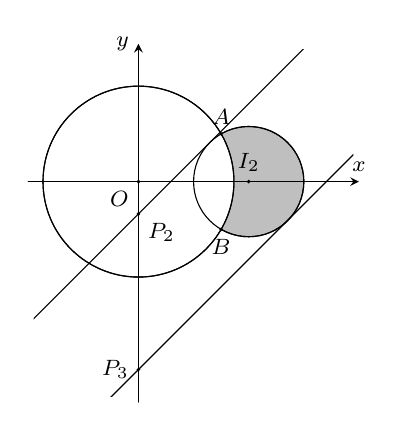
\begin{tikzpicture}[line cap=round, line join=round, font=\footnotesize, >=stealth, scale=.7]
			\draw[fill=gray!50] (2,0) circle(1cm);
			\draw[fill=white] (0,0) circle(1.732cm);	
			\def\xmin{-2} \def\xmax{4}
			\def\ymin{-4} \def\ymax{2.5}				
			\draw[->] (\xmin,0)--(\xmax,0) node [above]{$x$};
			\draw[->] (0,\ymin)--(0,\ymax) node [left]{$y$};
			\node at (0,0) [below left]{$O$};
			\clip (\xmin+0.1,\ymin+0.1) rectangle (\xmax-0.1,\ymax-0.1);
			\draw[smooth,samples=300] plot(\x,{1*(\x)-0.586});
			\clip (\xmin+0.1,\ymin+0.1) rectangle (\xmax-0.1,\ymax-0.1);
			\draw[smooth,samples=300] plot(\x,{1*(\x)-3.41});
			\draw (0,0) circle(1.732cm);	
			\draw (2,0) circle(1cm);
			\fill (0,0) circle (1.0pt) (2,3) circle (1.0pt) (0,-0.586) circle (1.0pt)node[below right]{$P_2$} (0,-3.41) circle (1.0pt)node[left]{$P_3$} (2,0) circle (1.0pt)node[above]{$I_2$} (1.5,0.866) circle (1.0pt)node[above]{$A$}(1.5,-0.866) circle (1.0pt)node[below]{$B$} ;			
			\end{tikzpicture}}
		Khi đó $ \heva{&x^2+y^2\ge 3\\&\log_{x^2+y^2}[x(4x^2-3x+4y^2)-3y^2]\ge 2} \Leftrightarrow\heva{&x^2+y^2\ge 3\\& (x-2)^2+y^2\le1.}$\\
		Gọi  $ D $ là miền giới hạn bởi phần bên ngoài đường tròn $ (C_1)\colon x^2+y^2= 3$ và phần bên trong đường tròn $(C_2)\colon (x-2)^2+y^2=1 $ kể cả bờ (Phần tô đậm như hình vẽ).\\
		Đường tròn $ (C_1) $ có tâm $ O(0;0) $ bán kính $ R_1=3 $, đường tròn $ (C_2) $ có tâm $ I_2(2;0) $ bán kính $ R_2=1 $.\\
		Giao điểm của hai đường tròn là $ A\left(\dfrac{3}{2};\dfrac{\sqrt{3}}{2} \right)  $ và $ B\left(\dfrac{3}{2};-\dfrac{\sqrt{3}}{2} \right) $.\\
		Xét họ đường thẳng $ \Delta $ song song $ x-y-P=0 $. Để thỏa mãn yêu cầu bài toán thì $ \Delta $ phải có điểm chung với miền $ D $.\\
		Gọi $ \Delta_1 $ là đường thẳng đi qua điểm $ A\left(\dfrac{3}{2};\dfrac{\sqrt{3}}{2} \right)  $ suy ra $ \dfrac{3}{2}-\dfrac{\sqrt{3}}{2}-P_1=0 \Leftrightarrow P_1=\dfrac{3}{2}-\dfrac{\sqrt{3}}{2}$.\\
		Gọi $ \Delta_2 $ là đường thẳng tiếp xúc với $ (C_2) $ do đó
		\begin{eqnarray*}
			\mathrm{d}[I_2,\Delta_2]=R_2	& \Leftrightarrow& \dfrac{|2-0-P|}{\sqrt{1^2+1^2}}=1\\
			&\Leftrightarrow & |2-P|=\sqrt{2}\\
			&\Leftrightarrow & \hoac{&2-P_2=\sqrt{2}\\&2-P_3=-\sqrt{2}}\Leftrightarrow \hoac{&P_2=2-\sqrt{2}\\&P_3=2+\sqrt{2}.}
		\end{eqnarray*}
		Với $ P=P_2 $ thì đường thẳng $ \Delta_2 $ không cắt miền $ D $.\\
		Ta thấy $ \Delta \cap Oy=(0;-P) $ do đó $ P_{\max}=P_3 =2+\sqrt{2}=M $ và $ P_{\min}=P_1=\dfrac{3}{2}-\dfrac{\sqrt{3}}{2}=m $.\\
		Vậy $ T=2(M+m)=2\left( 2+\sqrt{2}+\dfrac{3}{2}-\dfrac{\sqrt{3}}{2}\right)\approx 8{,}09  $.
	}
\end{ex}
\begin{ex}%[Đề thi thử THPT Yên Lạc 2 Vĩnh Phúc]%[Nguyễn Thành Nhân, 12EX-5-2223]%[2D1G3-1]
	Cho hàm số $ y=\dfrac{|\sin^2 x -(m+1)\sin x+2m+2|}{\sin x-2} $ (với $ m $ là tham số thực). Giá trị lớn nhất của hàm số đạt giá trị nhỏ nhất khi $ m $ bằng
	\choice
	{$ \dfrac{1}{2} $}
	{$ -1 $}
	{\True $ -\dfrac{3}{2} $}
	{$ -\dfrac{1}{2} $}
	\loigiai{
		Ta có $ y=\dfrac{|\sin^2 x -(m+1)\sin x+2m+2|}{\sin x-2}=-\left|\dfrac{\sin^2 x -(m+1)\sin x+2m+2}{2-\sin x} \right|=-\left| \dfrac{ \sin^2 x-\sin x+2}{2-x}+m\right|   $.\\
		Xét hàm số $f(x) = \dfrac{x^2-x+2}{2-x}+m$ trên đoạn $[-1;1]$. Ta có $f'(x) = \dfrac{-x^2+4x}{(2-x)^2} = 0 \Leftrightarrow \hoac{&x=0\\&x=4\text{ (loại)}.}$\\
		Ta có $f(-1) = m+\dfrac{4}{3}$, $f(0) = m+1$ và $f(1) = m+2$.\\
		Giá trị lớn nhất của hàm số đã cho là $\max\left\lbrace -\left| m+\dfrac{4}{3}\right| ,-|m+1|,-|m+2|\right\rbrace $.\\
		Ta thấy $m+1 < m+\dfrac{4}{3} < m+2$ nên $-\left| m+\dfrac{4}{3}\right|  < \max\{-|m+1|,-|m+2|\}$.\\ Do đó $\max\left\lbrace -\left| m+\dfrac{4}{3}\right| ,-|m+1|,-|m+2|\right\rbrace=\max\left\lbrace -|m+1|,-|m+2|\right\rbrace $.\\
		Đặt $A = m+1 = \left( m+\dfrac{3}{2}\right) -\dfrac{1}{2}$ và $B = m+2 = \left( m+\dfrac{3}{2}\right)  +\dfrac{1}{2}$.
		\begin{itemize}
			\item $m+\dfrac{3}{2} > 0 \Rightarrow \max\{-|A|,-|B|\} = -|A| > -\dfrac{1}{2}$.
			\item $m+\dfrac{3}{2} < 0 \Rightarrow \max\{-|A|,-|B|\}= -|B| > -\dfrac{1}{2}$.
			\item $m+\dfrac{3}{2} = 0 \Rightarrow \max\{-|A|,-|B|\} = -|A| = -|B| = -\dfrac{1}{2}$.
		\end{itemize}
		Vậy để giá trị giá trị lớn nhất của hàm số đạt giá trị nhỏ nhất thì $m =-\dfrac{3}{2}$.
	}
\end{ex}
\begin{ex}%[Đề thi thử THPT Yên Lạc 2 Vĩnh Phúc]%[Nguyễn Thành Nhân, 12EX-5-2223]%[2H1G3-2]
	Cho hình chóp $S.ABC$ có đáy $ABC$ là tam giác đều cạnh $3$. Các mặt bên $(SAB)$, $(SAC)$, $(SBC)$ lần lượt tạo với đáy các góc $30^\circ$, $45^\circ$, $60^\circ$. Biết hình chiếu vuông góc của $S$ trên mặt phẳng $(ABC)$ nằm bên trong tam giác $ABC$. Thể tích $V$ của khối chóp $S.ABC$ là
	\choice
	{$V = \dfrac{27\sqrt{3}}{2\left(4 + \sqrt{3}\right)}$}
	{\True $V = \dfrac{27\sqrt{3}}{8\left(4 + \sqrt{3}\right)}$}
	{$V = \dfrac{27\sqrt{3}}{4 + \sqrt{3}}$}
	{$V = \dfrac{27\sqrt{3}}{4\left(4 + \sqrt{3}\right)}$}
	\loigiai{
		\immini{
			Kẻ $SH \perp (ABC)$ tại $H$.\\
			Kẻ $HM \perp AB$; $HN \perp AC$, $HP \perp BC$. Ta có $\widehat{SMH} = 30^\circ$, $\widehat{SNH} = 45^\circ$, $\widehat{SPH} = 60^\circ$.\\
			Đặt $SH = x$, ta có:
			\begin{itemize}
				\item Tam giác $SHM$ vuông tại $H$ có $\widehat{SMH} = 30^\circ$\\ $\Rightarrow HM = \dfrac{SH}{\tan 30^\circ} = x\sqrt{3}$.
				\item Tam giác $SHN$ vuông tại $H$ có $\widehat{SMN} = 45^\circ$\\ $\Rightarrow HN = SH = x$.
				\item Tam giác $SHP$ vuông tại $H$ có $\widehat{SMP} = 60^\circ$\\ $\Rightarrow HP = \dfrac{SH}{\tan 60^\circ} = \dfrac{x\sqrt{3}}{3}$.
			\end{itemize}		
		}{
			\begin{tikzpicture}[font=\footnotesize,line join=round, line cap=round, >=stealth,scale=1]
			\path
			(0,0) coordinate (A)
			(0.8,-1.5) coordinate (B)
			(4,0) coordinate (C)
			(2,3) coordinate (S)
			(2,-0.5) coordinate (H)
			($(A)!0.4!(B)$) coordinate (M)
			($(A)!0.43!(C)$) coordinate (N)
			($(C)!0.45!(B)$) coordinate (P)
			;
			\draw (A)--(S)--(B)--(M)--(A) (C)--(B)--(A)--(M)--(S)--(P) (S)--(C);
			\draw[dashed] (A)--(C) (P)--(H)--(S)--(N)--(H)--(M) ;
			\foreach \x/\g in
			{S/120,A/180,P/300,B/200,M/180,N/145,C/0,H/45}\fill[black](\x) circle (1pt)($(\x)+(\g:3mm)$) node{\x};
			\end{tikzpicture}	
		}
		Mà $S_{ABC} = S_{HAB} + S_{HBC} + S_{HCA} \Leftrightarrow x\sqrt{3} + x + \dfrac{x\sqrt{3}}{3} = \dfrac{3\sqrt{3}}{2} \Leftrightarrow x = \dfrac{9\sqrt{3}}{2\left(3 + 4\sqrt{3}\right)}\cdot$\\
		Vậy thể tích khối chóp $S.ABC$ là
		$$V = \dfrac{1}{3}\cdot\dfrac{9\sqrt{3}}{2\left(3 + 4\sqrt{3}\right)}\cdot\dfrac{9\sqrt{3}}{4} = \dfrac{81}{8\left(3 + 4\sqrt{3}\right)} = \dfrac{27\sqrt{3}}{8\left(4 + \sqrt{3}\right)}\cdot$$
	}
\end{ex}
\Closesolutionfile{ans}
\begin{indapan}{10}
	{ans/ans-2-TT-25-YenLac2-VinhPhuc-L3-23}
\end{indapan}
